\chapter{Muestra y técnicas experimentales.}

\label{chap:techniques-and-sample}
\textit{En este capitulo discutiremos los principales aspectos de la muestra estudiada y las técnicas utilizadas para la 
caracterización de la misma.}
\vfill
\minitoc
\newpage

\section{Descripción de la muestra.}
\label{sec:chap3-sample-description}
Las muestras utilizadas son cristales de $ CdTe(001) $ y $ Hg_{0.18}Cd_{0.82}Te (001)$. En el caso del $ CdTe $ es una 
muestra no dopada intencionalmente ($ 5.6x10^{16} cm^{-3} $). En el caso del cristal de $ Hg_{0.18}Cd_{0.82}Te (001)$, este 
consiste de una capa de $ Hg_{0.18}Cd_{0.82}Te (001)$ de $ 1 \mu m $ de espesor crecida sobre un sustrato de $ CdTe(001) $. 
Las propiedades ópticas de ambos cristales han sido detalladamente estudiadas en los laboratorios del IICO por medio de 
Elipsometria Espectroscópica \cite{Camacho2005}\cite{LastrasMartnez2009}. El análisis y obtención de los parámetros ópticos 
han sido realizados tanto en el espacio directo como en el espacio inverso\cite{Camacho2005}\cite{LastrasMartnez2009}.

Es importante mencionar la importancia que estos materiales tiene en la configuración de sistemas que presentan fases de 
aislante topológico. Básicamente dos configuraciones han mostrado ser muy importantes, los pozos bidimensionales de de 
$ CdTe/HgTe/CdTe $ y el $ HgTe $ bajo tensión.

\subsection{Diagrama de bandas de CdTe y HgTe}
\label{sec:chap3-band-diagram}
El $ CdTe $ es un semiconductor directo cuya brecha fundamental a una temperatura de $300 K $ es $ E_{g}=1.44 eV $ 
\cite{Kittel2004-yd}\cite{Chadi1972}. Se muestra en la \ref{fig:band_diagram} (a) el diagrama simplificado de bandas en el 
punto $ \Gamma $ del centro de la zona de Brillouin\cite{Chadi1972}. La banda de valencia de los huecos ligeros y pesados 
tiene una simetría $ \Gamma_{8} $ y esta degenerada por 4. La banda \textit{Split-off} es de simetría $ \Gamma_{7} $ y 
degeneración 2. La banda de condición tiene una simetría  $ \Gamma_{6} $ y degeneración 2. En la misma figura se muestra 
las bandas para $ HgTe $ \cite{Chadi1972}.

Es importante notar, que el orden energético de las bandas  $ \Gamma_{6} $ y $ \Gamma_{8} $ no es el mismo para $ CdTe $ y 
$ HgTe $. Mientras que para $ HgTe $ la energía de la banda $ \Gamma_{6} $  es menor que para la banda  $ \Gamma_{8} $, para el 
$ CdTe $ el orden de las bandas es el contrario.

\begin{figure}[h!]
    \centering
    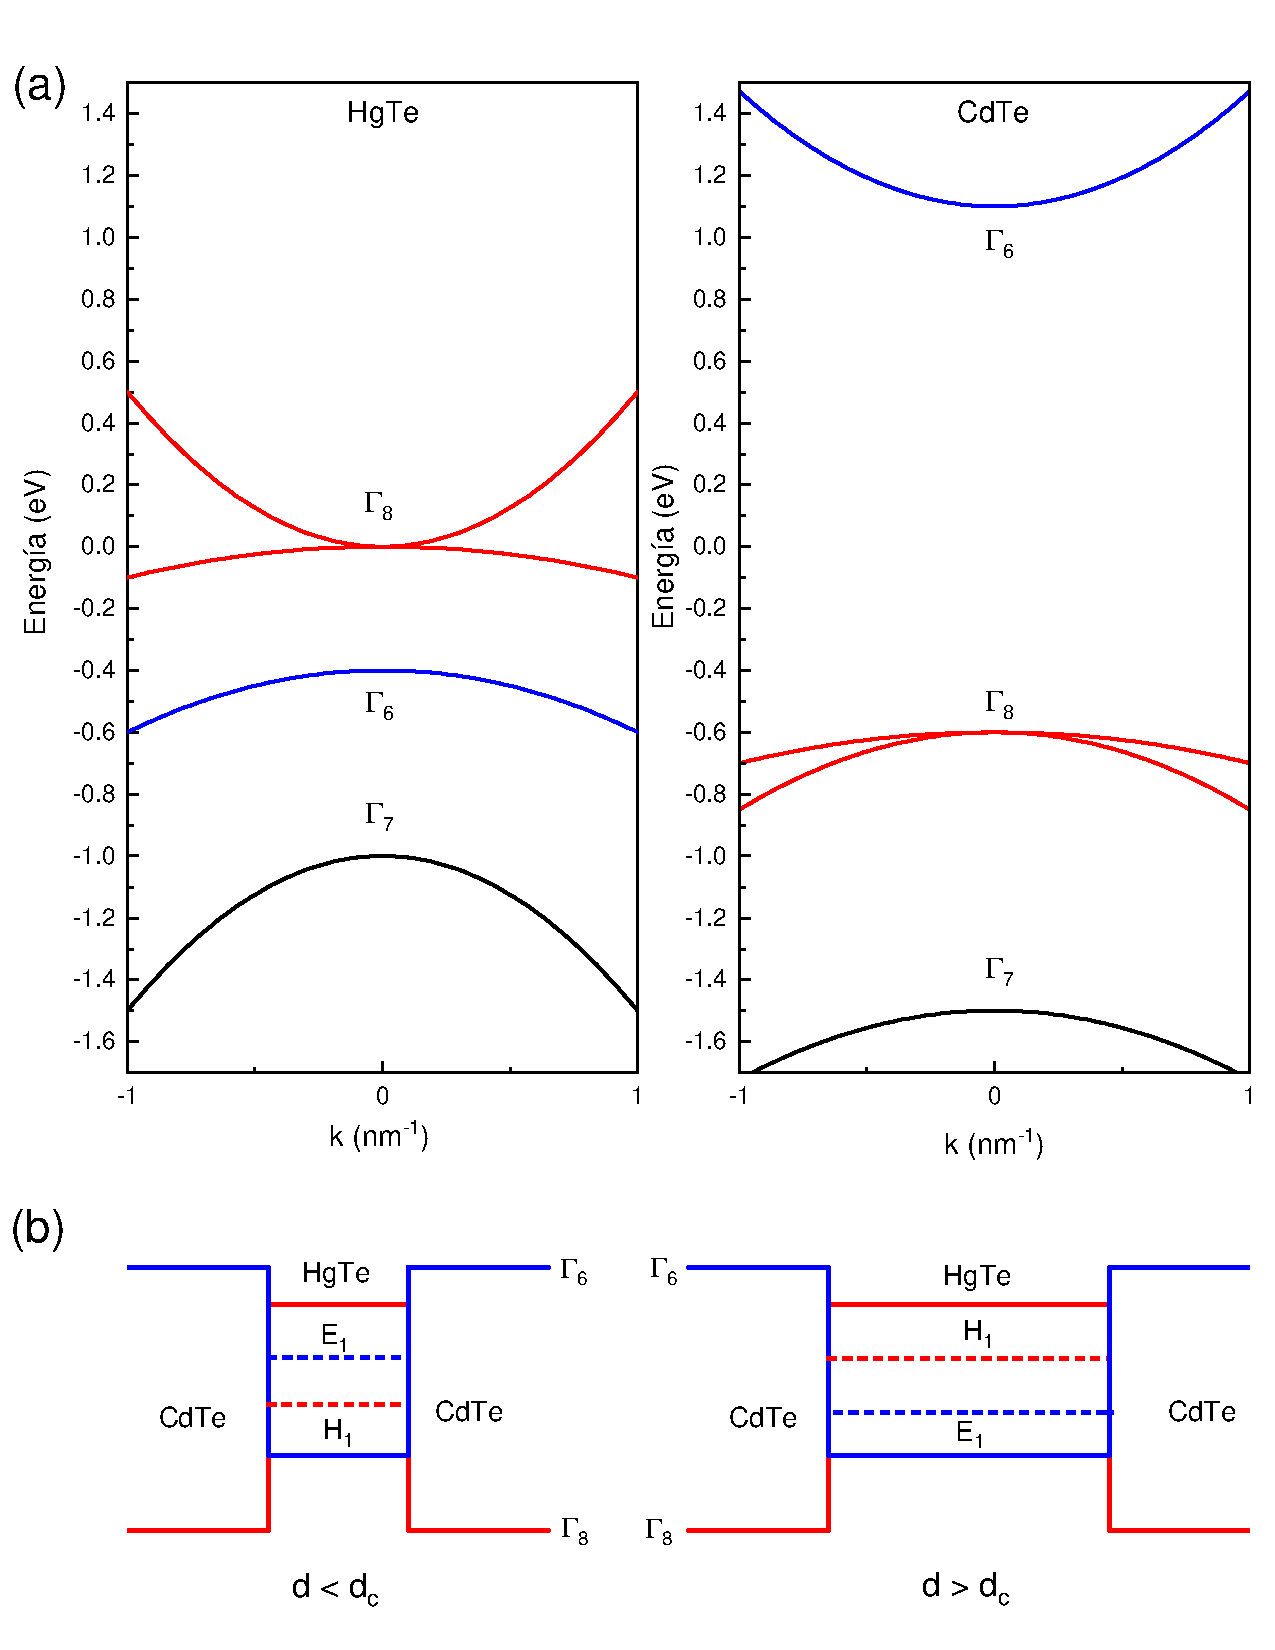
\includegraphics[width=0.8\textwidth]{figures/chap3/band_diagram.pdf}
        \caption{(a) Diagrama de bandas para los semiconductores $ CdTe $ y $ HgTe $. (b) Diagrama de bandas para el pozo
        bidimensional $ CdTe/HgTe/CdTe $ para diferentes casos de $ d = d_{c} $.}
    \label{fig:band_diagram}
\end{figure}

Lo anterior tiene consecuencias muy importantes en el caso de las estructuras de pozos basados en $ CdTe/HgTe $. Para 
comprender esta importancia se muestra en la \ref{fig:band_diagram} (b) un diagrama de las bandas de una estructura de pozos 
bidimensionales de $ CdTe/HgTe/CdTe $ \cite{Bernevig2006}. 
Para un cierto espesor \textit{d} del HgTe por debajo de un espesor critico $ d_{c} $, los niveles de los estados de los 
portadores $ E_{1} $ y $ H_{1} $ atrapados en el pozo tiene valores como los que se muestran, es decir $ E_{1}>H_{1} $. 
Al incrementar d por encima del valor crítico $ d_{c} $, las energías de los portadores evolucionan hasta llegar a la relación 
$ E_{1}<H_{1} $ en sus energías, es decir se produce una \textit{inversión} de las energías. Es evidente que 
en la condición $ d = d_{c} $ se cumple que $ E_{1} = H_{1} $. 

Este punto de inversión de las energías es también el punto de conversión entre un aislante convencional y un aislante 
topológico. Es decir, para \textit{d} > $ d_{c} $ el sistema presenta una fase topológica \cite{Bernevig2006}. 
Otra forma de manipular las bandas de energía en el $ HgTe $ y lograr fases topológicas, es por medio de la aplicación de 
una tensión. La tensión puede generarse a través del sustrato de $ CdTe $ sobre el que se crece el $ HgTe $ o aplicando 
la tensión externamente. En ambos casos, la degeneración de la banda $ \Gamma{8} $ es removida eliminando el carácter de 
semimetal del $ HgTe $ y produciendo una fase de aislante topológico \cite{Brne2011}\cite{Wu2014}. 

Otra forma de manipular las bandas de energía en el $ HgTe $ y lograr fases topológicas, es por medio de la aplicación de 
una tensión. La tensión puede generarse a través del sustrato de CdTe sobre el que se crece el $ HgTe $ o aplicando la 
tensión externamente. En ambos casos, la degeneración de la banda  $ \Gamma{8} $ es removida eliminando el carácter de 
semimetal del $ HgTe $ y produciendo una fase de aislante topológico \cite{Brne2011}\cite{Wu2014}. 

\section{Espectroscopia de Reflectancia Diferencial}
\label{sec:chap3-rds}
La técnica de Espectroscopia de Reflectancia Diferencial \textbf{(RDS)} es utilizada en el estudio 
de dispositivos y materiales, haciendo uso de la \textit{anisotropía}, la cual es la propiedad que 
describe como un material puede tener diferentes respuestas dependiendo de la dirección en la que es examinada, 
en este caso se debe a la \textit{anisotropía óptica}, donde observamos los cambios en la respuesta óptica 
del sistema estudiado, utilizando las propiedades de simetría y la polarización de la luz, para obtener 
una diferencia en la reflectancia del sistema observándolo de diferentes direcciones.

En el caso de los materiales semiconductores, nos aprovechamos de las propiedades
de simetría de los cristales observando dos direcciones cristalográficas, se elimina
la contribución del bulto o el cuerpo principal del semiconductor provocando que sea \textit{isotrópica}, 
obteniendo que la respuesta dependa solamente la superficie, haciendo que la \textbf{RDS} sea una 
técnica utilizada para el estudio de superficies.\cite{Aspnes1985} La respuesta o espectro de la 
\textbf{RDS} tiene la siguiente forma:

\begin{equation}
    \label{eqn:ch3-rds-eqn}
    {\Delta R} = \dfrac{R_{\alpha}-R_{\beta}}{2}
\end{equation}

Siendo $ \alpha $ y $ \beta $ las direcciones cristalográfica para las cuales se obtuvo la
reflectancia del material, siendo la diferencia de estos la que nos da la información de solamente la 
superficie.

\begin{figure}[h!]
    \centering
    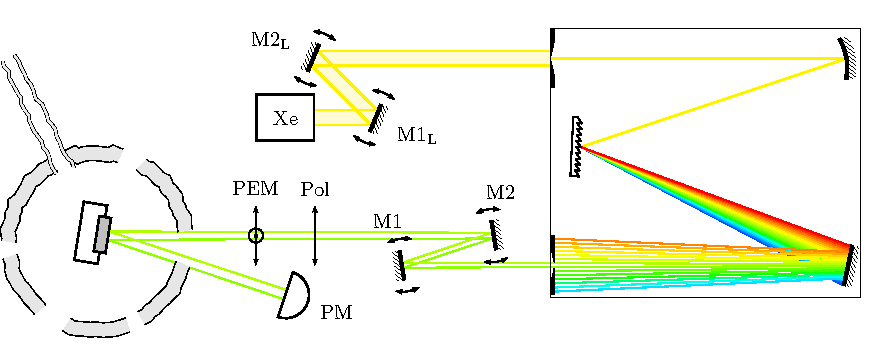
\includegraphics[width=0.5\textwidth]{figures/chap3/RAS-SETUP-gaby.pdf}
        \caption{Configuración utilizada para obtener los espectros de \textit{RDS} dentro de una Cámara de 
        Ultra Alto Vacío \textit{(UHVC)}.}
    \label{fig:rds-setup}
\end{figure}

El sistema utilizado para las mediciones tiene como fuente de iluminación una lampara de Xenón la cual es
enfocada hacia el monocromador con el uso de un arreglo de espejos, del cual sale la luz difractada dirigida a
otro arreglo de espejos los cuales dirigen la luz a la parte del sistema que controla su polarización, 
un prisma polarizador y un modulador fotoelástico que al pasar por ellos, obtenemos un haz de luz con 
una cierta polarización y que se estará modulando entre dos estados perpendiculares entre si, incidiendo sobre 
la muestra para reflejarse hacia un tubo fotomultiplicador.\cite{LastrasMartnez1993}

\section{Espectroscopia Raman}
\label{sec:chap3-raman}
La Espectroscopia Raman es una técnica que se aprovecha del \textit{efecto Raman}, el cual describe la interaccion
entre los fotones, el material que estamos estudiando y la forma en el que este vibra cuando los fotones incidan 
sobre una molécula, pudiéndose presentándose algún modo vibracional, siendo característico de la muestra, 
ya que esta estrechamente relacionado con la estructura molecular del material, resultando en la dispersión de 
fotones con diferentes frecuencias.\cite{Prasankumar2016}

\begin{figure}[h!]
    \centering
    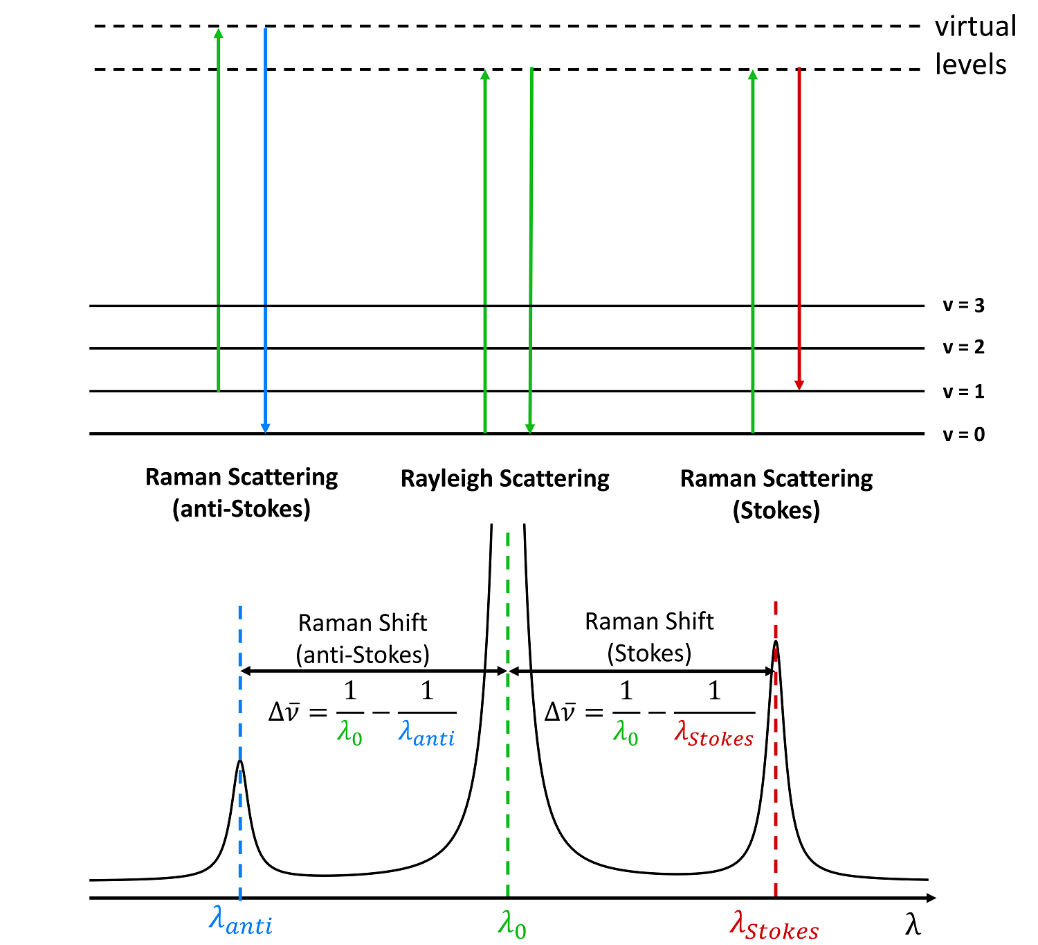
\includegraphics[width=0.7\textwidth]{figures/chap3/raman-ray-stokes-antistokes.png}
        \caption{Posibles resultados cuando un fotón choca contra la muestra, podemos observar la 
        dependencia de energía y el tipo interacción obtenida.}
    \label{fig:raman_diagram}
\end{figure}

Cuando un fotón choca contra una molécula puede ocurrir alguno de los siguientes casos:
    \begin{itemize}
        \item Que el resultado sea un choque elástico, queriendo decir que no perderá energía por medio de
        efectos vibracionales, dando como resultado un fotón dispersado con la misma frecuencia. Esto se conoce 
        como efecto Rayleigh.

        \item Que el choque resultante sea inelástico, lo que provoca que el fotón dispersado tenga una frecuencia 
        diferente a la del incidente, teniendo el caso de una mayor frecuencia, provocando una ganancia en la energía 
        con respecto al incidente y donde el fotón dispersado tiene menor frecuencia que el incidente, indicando que 
        ocurrió una perdida de la energía por procesos vibracionales. Estos son nombrados efecto Anti-Stokes y efecto 
        Stokes respectivamente.
    \end{itemize}

Por consecuencia, el efecto Stokes es utilizado para observar el \textit{efecto Raman}, siendo mas probable que
este suceda porque sus fotones dispersados tienen una energía menor que su contraparte del efecto Anti-Stokes.

En el caso de los semiconductores, debido a la existencia de la red cristalina, el efecto Raman nos puede dar información 
sobre la cristalinidad de la muestra, debido a que cada modo vibracional tiene una frecuencia para los fotones dispersados 
entre estos mas se alejen o apeguen de este valor nos da una noción de que tan cristalina es la muestra. Otra propiedad
importante es el entender el estrés al que esta sometido la muestra, por el desplazamiento de la respuesta del material 
en contraste con que no presente estrés.\cite{Weber2000}

En esta técnica, se utilizo el sistema comercial ***Nombre y marca del sistema***, el cual utiliza un laser de 633 nm
de potencia variable, con diferentes objetivos de 10x, 50x y 100x.

\section{Microscopia de Fuerza Atómica}
\label{sec:chap3-afm}
La Microscopia de Fuerza Atómica (AFM), es una técnica que es capaz de medir la superficie de un material a nivel 
nanométrico utilizando como principio las fuerzas de interaccion atractivas y repulsivas entre la punta del instrumento 
con el material. Para que la medición sea correcta, la punta debe tener una terminación en una cantidad de átomos 
pequeña, que al momento de experimentar una fuerza, esta provocara una deflexión en el cantiléver sobre el cual esta 
montada.\cite{Binnig1986}

\begin{figure}[h!]
    \centering
    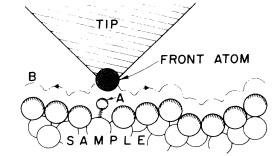
\includegraphics[width=0.7\textwidth]{figures/chap3/punta.png}
        \caption{Diagrama esquemático de la interaccion entre la punta de un sistema de AFM con una muestra, donde el 
        contorno \textit{B} representa el recorrido de la punta.\cite{Binnig1986}}
    \label{fig:afm_diagram}
\end{figure}

La configuración utilizada en este trabajo es conocida como \textit{modo tapping}, en el cual el cantiléver esta 
oscilando una cierta frecuencia, muy cercana a la de resonancia del mismo la cual es generada por un piezoeléctrico el 
cual genera vibraciones al aplicársele una corriente (\textit{piezoshaker}). El cantiléver esta oscilando en frecuencia 
y amplitud constantes cuando interactúa con la muestra, censando asi los cambios en estos dos parámetros para dar 
información sobre la muestra.\cite{Reifenberger2015-bh}

\section{Microscopía Óptica de Campo Cercano}
\label{sec:chap3-nsom}
***Pegar texto de Word***